\chapter{Introduction}

  \section{The chemical perception}
  Chemical perception is one of the oldest sensory systems, having evolved 500 million years ago. It mediated reproduction and feeding, two of the most fundamental animal behaviors. In fish, chemical perception passes through three distinct organs: olfaction, taste, and a common chemical sense. Unlike terrestrial species, where substances perceived by smell and taste differ by the medium of transport of the molecules, fish taste and smell through the same medium: water. The solubility of compounds in water determines the type of compounds that can be transported and perceived. The chemical perception is non-directional and persistent. The distance traveled and the perceived concentration depend on the diffusion and convection of the medium, determining the perception threshold and the compound's residence time in the environment. The chemical perception is extremely specific, being contained in the odorous compounds' molecular structures and the complex mixture of chemicals. Therefore, we expect to observe non-directional excitation behaviors or oriented gradient upward responses to find sources, such as orienting oneself or finding a place to lay eggs during migration. This navigation is a complex task and cannot be compared to a straightforward gradient ascent, as the aquatic environment is generally turbulent and perception is fragmented.

  The zebrafish larva is the model of choice for studying chemical directed navigation. In the larval stage, the animal is transparent. Therefore, it is possible to observe the entire brain with cellular resolution using light-sheet microscopy while the animal is performing a task and thus links behavior to neuronal activity. The sensory organs of chemical perception have been well characterized in the zebrafish. However, there are few behavioral studies on chemical perception and chemical oriented navigation. The model is widely used in addiction-related studies' due to the ease of genetic manipulations and its low cost. An animal model's characterization to study chemically oriented navigation, linking behavior to neuronal activity, would be a powerful addition to our understanding of how fish perceive and travel back to food sources, spawning and migration sites.

    \subsection{Olfaction}
    The olfactory organ of the fish Figure~\ref{olfactory_schematic} consists of two structures located in the animal's snout. Each structure consists of a cavity called the olfactory chamber connected to the outside by an entrance and an exit nostril. The inside of the olfactory chamber is lined with the olfactory rosette consisting of two rows of olfactory lamellae. The olfactory epithelium, where the olfactory receptors are located, is placed on these lamellae. The olfactory organ's exact organization and position can vary depending on the fish species, for example, with the addition of a ventilation cavity as an extension of the olfactory cavity.

    \begin{figure}[h]
      \centering
      \includegraphics[width=10cm]{part_2/assets/olfactory_schematic.png}
      \caption{Olfactory system, reproduced from \cite{hara2012fish}.}
      \label{olfactory_schematic}
    \end{figure}


    The olfactory epithelium has a $100\mu m$ thick stratified columnar structure. It can be separated into a sensory and a non-sensory epithelium. The sensory epithelium consists of three types of cells: receptor, supporting, basal cells, and the non-sensory epithelium of Goblet cells and non-sensory ciliated cells. The receptor cells are ciliated cells, microvillous cells, crypt cells \cite{ichikawa1977fine,hansen2005diversity}, kappe cells \cite{ahuja2014kappe}, and pear cells \cite{wakisaka2017adenosine} that express olfactory receptors of the OR, V1R, V2R, and TAAR families. receptor cells have various sizes, shapes and places inside the epithelium see Figure~\ref{olfactory_schematic_full} Receptor cells project directly into the olfactory bulb located in the brain, in turn sending signals to the telencephalon and diencephalon \cite{miyasaka2009olfactory}.

    \begin{figure}[h]
      \centering
      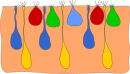
\includegraphics[width=10cm]{part_2/assets/olfactory_schematic_full.png}
      \caption{{\bf Schematic representation of the olfactory epithelium.} Ciliated neuron in yellow with round somata, slender dendrite, and cilia. Microvillous neuron in dark blue with microvilli at the surface. Crypt neuron in red with ovoid shape, microvilli, and cilia. Kappe neuron in green with microvilli. Pear-shaped neuron in light blue with cilia.}
      \label{olfactory_schematic_full}
    \end{figure}

    The olfactory bulb in the teleost is a structure of four concentric layers: olfactory nerve layer (ONL), glomerular layer (GL), mitral cell layer (MCL), and internal cell layer (ICL). The olfactory information is transmitted by the receptor cells to the olfactory bulb \cite{nikonov2001electrophysiological} then in the forebrain \cite{nikonov2005beyond} as a topographical odor map. The olfactory bulb's neuronal connections have been particularly studied in zebrafish \cite{hansen1998peripheral,kermen2013neural}. Each receptor cell expresses only one type of olfactory receptor \cite{serizawa2004one,barth1997noncoordinate,weth1996nested,sato2007hierarchical} except in a subpopulation of olfactory sensory neurons \cite{sato2007hierarchical}. Cells expressing the same receptor are projecting into the same olfactory bulb glomeruli \cite{sato2005mutually}. The olfactory bulb of the zebrafish comprised approximately 20 000 neurons \cite{friedrich2009processing} and 140 glomeruli\cite{braubach2012distribution}. Glomeruli responding to similar odorants are grouped into domains within the olfactory bulb, forming chemotopic maps. Odorants can activate glomeruli outside their domain, leading to a fragmented map inside the olfactory bulb \cite{friedrich1998chemotopic}. Moreover, the odor encoding is hierarchized with first-order features encoded by large domains and second-order features by local activity patterns within the domain \cite{fuss2001odorant,korsching2001odor}.

    The olfactory bulb projects into two higher brain structures, the telencephalon (Dp and Vv) and the diencephalon (habenula, posterior tubercle, and hypothalamus). Odor response in these areas is currently poorly understood.

    In the zebrafish \cite{hansen1993development,miyasaka2013functional}, the olfactory organ develops from the olfactory placodes at the 6-10 somites stage (about 15 hours post-fertilization) of embryonic development. The olfactory cavity begins to appear at the 28-30 somites stage (31 hours post-fertilization). Approximately 50 hours post-fertilization, the olfactory epithelium and the receptor cells appear. When the embryo emerges from the egg, 4 days post-fertilization, the olfactory organ continues its morphological development, but the cytological organization changes little. At 40 days post-fertilization, the bridge between the entrance nostril and the exit nostril is completely formed, separating the currents going out and coming in from the olfactory cavity. The addition of lamellae to the olfactory rosette continues throughout the life of the zebrafish.

    \subsection{Gustation}
    The gustatory organ of fish consists of the taste buds, which directly contact chemical substances.
    Taste bud histology has been studied for different fish \cite{kapoor1976gustatory,fishelson2004taste,reutter2000heterogeneity,reutter1991ultrastructure,reutter2012taste}. Taste buds usually have an elongated and ovoid shape. They extend throughout the thickness of the epidermis and protrudes from the surface. They sit on a small dermal papilla. The taste bud is constituted of a sensory (dark cells with microvilli, and light cells with one large microvillus) and a non-sensory epithelium (Merkel‐like basal cells). The apical ending of the sensory cells that protrude from the epithelium is called the receptor field and covers with a mucous cap. The number of sensory cells in a taste bud varies considerably depending on the fish species.
    Taste buds are distributed all over the fish's body, especially in the mouth, on the lips, and the skin. Their distribution and concentration vary according to the species. Three different cranial nerves innervate them: facial (VII), glossopharyngeal (IX), and vagal (X). The facial nerve transmits information from the extra-oral taste buds; the glossopharyngeal nerve transmits information from inside the oral cavity; the vagal nerve transmits information from inside the oropharyngeal cavity. The taste system is anatomically divided into two distinct parts: nerves IX and X projecting into the brain's vagal lobe and nerve IV into the facial lobe. Connections to higher areas of the brain differ slightly from one species to another. It has been shown in Ictalurus nebulosus \cite{datema1971structures} that these two systems have distinct roles in fish feeding behavior.

    \begin{figure}[h]
      \centering
      \includegraphics[width=8cm]{part_2/assets/gustatory_schematic.png}
      \caption{\textbf{Schematic drawing of a typical taste bud of teleosts from \cite{hansen2002taste}.} Dark cells (Cd), light cells (Cl) and Merkel‐like basal cells (Cb). Marginal cells (Cm). Ce epithelial cells. Dermal papilla (DP). (TBN) taste bud nerve. (BL) basal lamina. (RA) receptor area. (VC) capillary vessel.}
      \label{gustatory_schematic}
    \end{figure}

    In zebrafish \cite{ohkubo2005distribution}, the taste buds (approximately 2 200) are located on the lips, in the oropharyngeal cavity on the barbels, and on the head's ventral and dorsal side. Each taste bud contains $20 - 23$ cells. Projections of the zebrafish gustatory system have been studied in detail \cite{yanez2017gustatory} and form a complex network that can be summarized graphically on Figure~\ref{gustatory_connection_schematic}.

    \begin{figure}[h]
      \centering
      \includegraphics[width=10cm]{part_2/assets/gustatory_connection_schematic.png}
      \caption{\textbf{Gustatory system of the zebrafish}. Neuronal connections of the fish taste system reproduced from \cite{yanez2017gustatory}.}
      \label{gustatory_connection_schematic}
    \end{figure}

    The development of the gustatory organ has been studied in the zebrafish \cite{hansen2002taste}. The first taste buds appear at 3 or 4 days post-fertilization and are located on the lips and the gill arches. The taste buds in the mouth and oropharyngeal cavity appear 4 to 5 days post-fertilization. The taste buds on the head do not appear until 12 days post-fertilization, and it is not until the juvenile stage (30 to 40 days post-fertilization) that the barbels appear. Note that the appearance of the taste buds coincides with the appearance of feeding in the larvae.

    \subsection{Commom  chemical sense}
    Fish also have a third chemical sense called the common chemical sense. It consists of bipolar cells called solitary chemosensory cells (SCCs) present in the epidermis. Their distribution and number vary greatly depending on the species. Therefore their study is difficult, and their function and neuronal connection are poorly understood. SCCs are embedded in the fish epidermis and comprised of bipolar sensory neurons.

    In the zebrafish \cite{kotrschal1997ontogeny}, SCCs have been described as either a set of 2-7 villi of 0.5 to 1 $\mu m$ length emerging from the cell body at embryo and larval stage.  Alternatively, in adults, SCCs possess a single villus of $3\mu m$ length.

    The first SCCs appear at 3 days post-fertilization. Their density increases until 25 days, where their number stabilizes at $1.10^6$ per $mm^2$ with 2 to 5 times more SCCs on the zebrafish's head than on its body.

    \subsection{Behavior}
    The olfaction and gustation have been shown to mediate several fish behaviors. It is not easy to distinguish the contribution of each sense in the observed behavior. Moreover, this contribution seems to be dependent on fish species.

    A well known and impressive behavior encountered in many fish species is the homing migration. A typical example is salmons that perform three migratory phases throughout their life. One of them, the upstream migration from the ocean to their home stream, has been shown to rely on an olfaction imprinting \cite{stabell1992olfactory, hasler1983olfactory}. Little is known about the imprinting mechanism, but experiments suggest that it relies on a mixture of odors perceived during the juvenile stage in the fish's home stream.

    Feeding is one of the most important behaviors. It relies on several senses for food detection, and selection \cite{pavlov1990sensory}. A stereotyped behavioral sequence was shown to exist \cite{atema1980chemical} consisting in a step of arousal mainly mediated by olfaction \cite{bateson1890sense}, then a step of localization of the food mediated by chemical and visual cues. The last step of ingestion is triggered primarily by the gustation \cite{atema1980chemical}. The impact of each sensory modality varies significantly with the species. For example, the yellow bullhead has the entire feeding sequence mediated by taste, whereas ictalurid catfish prey detection was abolished when olfaction was blocked. The chemical substances that attract fish depend on the species \cite{atema 1982}, and response to a mixture is higher than isolated compounds in general.

    Olfaction \cite{tavolga1956visual} as well as the gustatory system \cite{de1983influence} has been shown to play an essential role in reproduction. Non-anosmic males exposed to water taken from a tank with a gravid female developed courtship behaviors, except for some species like the three-spined stickleback where the gustation can replace the olfaction. Complete courtship repertoire necessitated the presence of other sensory cues.

  Fright reaction occurred when a fish perceived an alarm substance secreted by a conspecific. This reaction differs between species and involves seeking cover, rapid swimming, or freezing. It is accepted to be mediated by olfaction \cite{frisch1942schreckstoff,speedie2008alarm,doving2009alarm}, but other sensory cues are not ruled out.

  \section{Behavioral studies}
  The zebrafish remains the model of choice to study the behavioral response to diverse stimuli.  They are used to study behaviors such as response to visual stimuli \ref{}, heat \ref{}, and the study of balance reflexes \ref{}. It is transparent at the larval stage, and therefore the entire brain can be observed through a light-sheet microscope using genetically modified lines \ref{}. In theory, we can efficiently study the link between response to a stimulus and neuronal activity.
  For the chemical perception, few studies have been done on zebrafish larvae, most of the work being focused on drug screening with a medical focus in mind. The behavioral study of the chemical perception of zebrafish, adults, or at the larval stage has been done through various experimental apparatus that we will present in the following sections.

    \subsection{Conditioned place preference}
    Conditional place preference (CPP) is a type of Pavlovian conditioning. It consists of associating a conditioned stimulus that has been taught to the animal with an unconditioned stimulus that one seeks to test. The most classic example is associating the sound of a bell with the release of a food smell. After learning, the animal can responds to the conditioned stimulus alone.
    This classical psychology approach has been applied in adult zebrafish to test the response to various chemical stimuli \cite{mathur2011conditioned}.

    Experiments follow a 3-step design.
    The first step is to evaluate the fish's preference. The fish is placed in a separate aquarium in two or three parts. Each part has walls with a different pattern and color. The fish is tested to find out which side it naturally prefers. Usually, fish with strong preferences are eliminated.
    The second step is the conditioning phase. The fish is restrained to its least preferred aquarium side and the substance to be tested injected in the water. This step can be repeated several times if necessary.
    The last step consists of repeating the first step to assess the change in preference of the animal.

    With this method, \cite{darland2001behavioral} studied the sensitivity of cocaine on adult zebrafish. They showed a strong and robust cocaine-induced CPP response in WT fish, with $85\%$ of the fish changing preference to a cocaine concentration of $10mg.L^{-1}$. Lower and higher concentrations result in a lower response.
    \cite{mathur2011preference} studied the response of adult zebrafish to ethanol in a device with two chambers with different patterns and a central alley with a uniform pattern allowing the fish to be placed first in a neutral environment. The experiment lasted two days. For the first day, the preference of each fish was access from a five minutes recording. On the second day, each animal was conditioned with ethanol in its least preferred side for 20 minutes, and in the preferred side with just water. The experiment was done by alternating the order of the two conditionings. On the third day, the preference of each animal was reaccessed from a five minutes recording. The authors show a positive response to the conditioning at a concentration of $1.5\%$ of ethanol without significant effect of the conditioning order. It should be noted that this is also the first study to use an automated tracking system to calculate animal preference.
    Similar experiments were performed to test the response to various chemical stimuli. \cite{ninkovic2006genetic, ninkovic2006zebrafish} showed a positive response to CPP for D-amphetamine; \cite{braida2007hallucinatory} show a positive response to salvinorin A, cocaine, and spiradoline; \cite{kedikian2013behavioral, } show a positive response of CPP to nicotine and ethanol.

    \subsection{Well-plate}
    A widely used experimental device to quantify a chemical compound's effect on zebrafish larvae is the well-plate device. A zebrafish larva is placed in each well, and a chemical compound is diluted into the well. The larvae are then recorded swimming in the chemical compound, and the kinematic parameters of the animal are extracted. The advantage of this technique is that it requires little equipment. It quickly produces a large amount of data with well-plate up to 48 wells per plate. Software already exist to extract relevant behavior parameters from video recording automatically. With this device, many chemical compounds have been tested \cite{sallinen2009mptp,rihel2010zebrafish,kokel2010rapid}, seizure liability \cite{winter2008validation}, avoidance behavior \cite{pelkowski2011novel}, swimming behavior \cite{farrell2011evaluation}.

    \subsection{Diffusion}
    Some authors have tried to quantify chemical, behavioral effects by introducing a chemical compound directly into the aquarium and looking at the percentage of time spent close to the source. Notably, \cite{wakisaka2017adenosine} showed an attraction concentration-dependent to adenosine for adult zebrafish. The ATP and ADP, naturally produced by living organisms, are dephosphorylated in the fish's olfactory epithelium. The resulting adenosine is perceived by a sensory cell that they discovered and called pear-shaped cell that expresses specific receptors for adenosine. \cite{krishnan2014right} showed in zebrafish larvae a concentration-dependent attraction to GCDA and nicotine using an aquarium with two compartments and an intermediate zone where the fish can choose changes compartment. \cite{hussain2013high} show with a system close to \cite{krishnan2014right} a strong aversion to cadaverine, an odor associated with decomposing bodies.

    This type of experimental device's weak point is the lack of control in the real concentration of product perceived by the animal. Diffusion and convection are neglected in the experiments, and the concentration perceived by the animal is poorly known and not reproducible. \cite{hussain2013high,krishnan2014right} mitigates the effects of diffusion and convection with a wall separating the two zones, always leaving uncertainty in the intermediate zone. Moreover, these montages exclude the realization of long experiments due to the homogenization of the concentration by diffusion.

    \subsection{Flow}
    Another class of device to study the chemical perception of fish is an underflow device. Various experimental set-ups have been reported in the literature without a standard emerging to compare the results.
    \cite{abreu2016acute, abreu2016behavioral} uses a laminar flow device to separate an aquarium into two distinct compartments without a physical wall. The first mention of this type of device date back to 2013 \cite{readman2013fish}. The animal can then choose between the two compartments without constraints. The interface between the two virtual compartments self-heal with a characteristic time depending on the flow velocity, mitigating the convection problem mentioned previously. Several psychoactive substances have been tested on adult zebrafish. The time spent in the product, the number of crosses and the animal's kinematic parameters are extracted from video recordings. They show attraction by diazepam, fluoxetine, risperidone, and buspirone; an aversion to acid pH and two food odor extracts; a neutral behavior for ethanol. They found no change for the kinematic swimming parameters, except for the two food odor extracts. Always with the same experimental device, the authors tested the attraction or repulsion to conditioned water. First, fish are placed in an aquarium and subjected either to chemical stress (decrease in pH), physical stress (hunting by a net), predator image, or finally to more or less food deprivation. In a second step, fish are tested in the laminar flow device with normal water on one side and conditioned water from the first step on the other side. The authors find a significant aversion to water conditioned by chemical and physical stress. No significant difference was found for predator image conditioning. They showed an aversion to water conditioned with fish deprived of food for 48 hours and no difference for fish following regular feeding or chronic fasting.

    \cite{kermen2020stimulus} used a flow device that, instead of separating the aquarium into two compartments, allows the concentration of the product in the entire aquarium to be quickly changed. By recording the animal's kinematic parameters, they can then conclude on the impact of the chemical compound. The results are no longer expressed this time in terms of attraction-repulsion but can be compared to those of the well-plate, the interest being to experiment with adult animals that require a large volume of water in three dimensions to evolve realistically. With this device, the authors show that the fish modulate their trajectory by modulating seven independent parameters: speed, number of bursts, number of turns, horizontal and vertical displacement, time spent frozen, and the vertical position. From these metrics, they can classify the odors by grouping them by similar behavioral responses. They found that food odors resulted in a significant increase in speed and number of burst; social odors (from other fish) resulted in a similar response to food odors; alert odors result in a descent to the bottom of the aquarium and an increase in frozen time; decomposition odors result in more turns.
    The critical points noted by this study is the inter-and intra-experimental variability. The authors showed that less than a third of the odors used in the study produce reproducible results between trials of the same individual. Some odors such as cadaverine, blood, skin, and food odors resulted in inconsistent responses for the same individual. Most odors produce poorly reproducible results for different fish.

    This type of experimental device allows better management of the concentration perceived by the animal, which is perfectly controlled after a transient regime. It also allows the realization of long experiments, as the flux allows to stop the diffusion and convection of the chemical compound.

    Therefore, we can see from this overview of the scientific literature that the study of chemical perception and behavioral response to chemical stimuli is not standardized. No experimental set-up is set as a standard and does not allow a direct comparison between studies carried out in various independent laboratories. It is in this context that we have developed Dual. This experimental set-up is easy to construct, well documented, and allows the study of the behavioral response in larvae and juvenile zebrafish in a standardized and comparable way.


\chapter{Dispositif expérimental}

  \section{Dual}
  \subsection{Introduction}
  La reproductibilité des études comportementales est un problème ouvert en neuroscience. La conception et la réalisation de montages expérimentaux permettant un grand débit d'expériences en d'éviter tout biais est essentielle à la caractérisation d'un comportement. L'absence de standard en matière d'étude de la réponse comportementale à des stimuli chimiques ne permet pas à ce jour de comparer facilement les résultats obtenus au travers des diverses études menées jusqu'à présent. C'est dans ce contexte que nous présentons Dual, un montage expérimental à haut débit d'expérience facile à réaliser et à mettre en place.
  \medbreak
  On verra dans un premier temps la philosophie du dispositif, dans quel but il a été conçu et pour quelle utilisation. Dans un second temps les étapes de construction et enfin on verra son utilisation et son coût en temps pour réaliser une campagne d'expérience.
  \subsection{Philosophie}
  Dual est un système du même type que \cite{readman2013fish} qui consiste à créer grâce à un flux laminaire deux compartiments virtuels dans l'aquarium. Comme on l'a vu précédemment, ce système permet une connaissance rigoureuse de la concentration du composé chimique auquel est soumis l'animale. Il permet aussi d'éviter la convection due au mouvement d'eaux engendré par la nage du poisson, toutes les perturbations étant entraînées par le flux. On a donc deux compartiments virtuels bien défini par une interface qui se "répare" d'elle-même dans un temps caractéristique donné par la vitesse de l'écoulement laminaire. 
  \medbreak
  Pour se faire, Dual utilise un système de quatre seringues (2 seringues infectantes et 2 seringues aspirantes) qui permet de créer un flux laminaire constant dans l'aquarium où évolue le poisson. Le rôle des seringues peut être inversés grâce à un système de valves pour pouvoir les remplir et choisir le produit qu'elles contiennent. On peut alors construire une expérience en réalisant plusieurs cycles de remplissage-injection. Par exemple en aspirant en premier de l'eau dans les deux seringues ce qui constituera en injection un flux laminaire d'eau homogène (contrôle) et dans un second temps un produit dans une seringue et de l'eau dans l'autre ce qui en injection permettra de créer un flux laminaire de produit et un flux laminaire d'eau créant deux compartiments virtuels dans l'aquarium. 
  \medbreak
  Dual est inspiré du mouvement Do It Yourself qui permet de construire des choses sans l'aide d'expert du domaine. C'est dans ce sens que tous les composants, plans et autres fichiers CAD nécessaires à la création et au montage de Dual sont disponibles en annexe. Dual peut être construite à moindre coût sans connaissance préalable en mécanique ou en électronique. Les machines nécessaires à la réalisation des pièces peuvent être trouvé dans un FabLab et à moindre coût.
  \subsection{Construction}
  \paragraph{Overview}
  Dual est constitué de quatre parties distinctes : une partie mécanique, une partie hydraulique, une partie électronique et enfin un logiciel informatique permettant de contrôler tout le dispositif.
  \paragraph{Système mécanique}
  La partie mécanique de Dual comprend un pousse seringue motorisé, un support de caméra et un aquarium isolé de l'environnement extérieur. Le pousse-seringue motorisé permet d'accommoder quatre seringues figure~\ref{} qui marche deux à deux en opposition de phase. Quand les seringues supérieures injectent, les seringues inférieures se remplissent et inversement. Cela va permettre de créer le flux laminaire nécessaire à la création des deux compartiments virtuels. Tous les plans et fichiers nécessaires à la réalisation des différents éléments est disponible en annexe.
  \medbreak
  L'aquarium figure~\ref{} est constitué d'une puce millifluidique en XXXX réalisée à la découpe laser et coller grâce à de l'acide acétique. Le XXXX est un matériau plastique transparent ce qui permet de conserver une bonne qualité d'image quand on filme en transmission. Elle est constituée en son centre d'une zone délimitée par deux grilles en plastique réalisées en impression 3D où le poisson pourra évoluer. La puce comprend deux entrées et deux sorties qui seront connectées par le système hydraulique aux seringues. Cela permet de créer deux flux laminaires à volume constant dans l'aquarium. Le tronçon reliant les entrées et les sorties à la zone où le poisson est confinée présente un profil évasé pour éviter toutes perturbations et un raccordement optimal entre les deux flux laminaires. Enfin, une plaque en plastique est placée au-dessus du système et permet d'éviter que le poisson ne s'échappe et les déformations optiques lors de l'enregistrement.
  \medbreak
  La puce millifluidique est placée dans une boîte réalisée avec une structure en MakerBeam et des panneaux en MDF découpé à la découpe laser. Cette boîte permet d'isoler l'expérience du milieu environnant et de placer l'animale dans un éclairage contrôlé (ou bien obscurité complète). Cette boîte contient figure~\ref{} de bas en haut : deux LED permettant d'éclairer en lumière visible et en infrarouge (nécessaire pour l'enregistrement), un diffuseur permettant un éclairage homogène, la puce microfluidique et sur la face supérieure une fenêtre amovible constituée d'un filtre laissant uniquement passer la lumière IR, cela permet de bloquer toutes lumières extérieures tout en pouvant enregistrer les images de l'expérience en lumière IR.
  \medbreak
  Un support de caméra est placé au-dessus de la boîte et une caméra Chameleon3 FLIR Systems permet d'enregistrer les expériences en lumière IR.
  \medbreak
  Tous ces éléments sont fixés solidement et à niveau à la table pour éviter toutes vibrations ou biais qui pourraient perturber l'animale pendant l'expérience. La facilité de réalisation de la puce microfluidique en moins de 12 h permet de la remplacer facilement en cas de détérioration ou de contamination.
  \paragraph{Système hydraulique}
  Le système hydraulique permet de relier les seringues à la puce microfluidique avec un système de valves permettant de choisir quelle seringue injectera dans quelle entrée de la puce microfluidique, et depuis quel récipient se remplira la seringue, un schéma du circuit est disponible figure~\ref{}. Ce système permet de créer des expériences construites en mettant bout à bout des cycles de remplissage et d'injection. Les valves sont contrôlées électroniquement ce qui permet d'automatiser complétement le système.
  \paragraph{Système électronique}
  Le système électronique permet de faire l'interface entre les éléments à contrôler que sont les valves, les LED et le moteur du pousse-seringue et le logiciel informatique. Le circuit imprimé a été créé sur-mesure~\ref{}. Il accueille un Arduino Nano servant de microcontrôleur, Six relais permettant le contrôle des valves à partir des signaux logiques de l'Arduino. Un contrôleur de moteur pas à pas EasyDriver permettant de contrôler la vitesse du moteur depuis une sortie logique de l'Arduino. Un système de potentiomètre permet de contrôler l'intensité des LED d'éclairage. Tout le système électronique ainsi que le moteur du pousse-seringue est alimenté par une alimentation ATX d'ordinateur 550W connectée au circuit imprimé par un montage inspiré du Benchtop Power Board de Sparkfun.
  \paragraph{Système informatique}
  Un logiciel a été développé spécialement pour contrôler le dispositif. L'interface graphique a été créée à l'aide de Qt et la caméra est interfacé au logiciel grâce au SDK de FLIR Systems. Le logiciel permet de contrôler manuellement chaque élément du système comme les valves, la caméra et le moteur du pousse-seringue. Il permet de contrôler l'éclairage ainsi que d'enregistrer les images provenant de la caméra. Il est possible (et conseillé) de créer des templates d'expériences, un simple fichier texte, contenant les instructions nécessaires à l'automatisation des cycles d'injection et d'aspiration. Le logiciel permet de contrôler depuis la même interface quatre Duals.
  \subsection{Utilisation}
  Pour nos besoins, nous avons construit quatre Duals que nous avons fait tourner en parallèle. La construction complète du montage nécessite une découpe laser, une imprimante 3D, du matériel électronique (fer à souder, etc.) et du matériel d'atelier (tournevis, vis, perceuse, etc.) et les matériaux et plan (disponible en annexe ~\ref{}. Deux semaines ont été nécessaires à la construction du dispositif à partir des plans. La construction ne demande pas de connaissance spécifique et la construction par exemple dans un FabLab permettra de trouver le matériel et l'aide nécessaire en cas de difficultés à réaliser le projet.
  \medbreak
  L'utilisation du Dual est extrêmement simple en pratique. Une fois le template d'expériences créé, la seule tâche manuelle est de placer le poisson dans la puce microfluidique, de refermer le dispositif et de faire jouer le template d'expérience. Il est nécessaire de contrôler que les récipients d'aspiration (eau où produit) sont remplis. Il est alors possible d'enchaîner les expériences avec peu de temps mort et une intervention manuelle minimale.
  \medbreak
  Un problème récurrent que nous avons rencontré est l'encrassage du circuit hydraulique. Le colorant utilisé pour visualiser l'écoulement~\ref{} fini par boucher les valves. Une solution trouvée est de régulièrement passer les valves dans un bain ultrasonique pour les déboucher et de changer de temps en temps les tuyaux qui raccordent les valves, les seringues et la puce microfluidique. Le fait d'effectuer un protocole de rinçage qui peut être lancé automatiquement à la fin de la journée nous a aussi permis de réduire ce problème. 

  \section{The Tropical River}
  \subsection{Description}
  La perception chimique dans un environnement aquatique turbulent comme lequel sont soumis les poissons nécessite un dispositif expérimental permettant de créer de manière contrôlé des écoulements et de délivrer des stimuli chimique. Pour se faire, nous avons créé un dispositif expérimental permettant de délivrer un écoulement laminaire à température contrôlée, permettant d'imager les poissons aussi bien en lumière visible qu'en lumière infrarouge pour les placer dans le noir total. Une buse d'injection permet de créer des panaches turbulent ou laminaire à l'intérieur de cet écoulement.
  \paragraph{Dispositif mécanique}
  La partie mécanique du dispositif est constitué d'un canal assemblé à partir de plaque de PVC transparent. Une plaque lumineuse est placé sous le canal permettant un éclairage en lumière visible par le dessous pour éviter toutes réflexions sur la surface de l'eau. Le canal peut être éclairé par le dessus par un ensemble de LED infrarouge. Une caméra est placée au-dessus du canal et permet d'enregistrer les expériences. Un miroir est placé à 45 degrés sur le côté du canal ce qui permet de récupérer les positions verticales des poissons sur la même image que leurs positions horizontales. L'ensemble du canal est placé dans une boîte pour l'isoler de la lumière et de toutes perturbations liées à l'environnement immédiat de l'expérience.
  \paragraph{Dispositif hydrodynamique}
  Le canal est alimenté en eau depuis un robinet connecté au réseau d'eau du bâtiment. Avant d'arriver dans le canal, elle est filtrée par un filtre au charbon actif, chauffé grâce à un système de bain marie puis injecté par une extrémité du canal. Un réseau de paille est placé dans le canal permettant ainsi de régulariser l'écoulement turbulent en écoulement laminaire. Le débit peut être ajusté grâce à une valve solénoïde. L'autre extrémité du canal est laissé libre et l'eau sortante est redirigé vers le réseau d'eau usé du bâtiment, les produits testés ne nécessitant pas de traitement particulier. Il est possible de diluer un produit en amont du canal grâce à une buse d'injection située directement à la sortie de l'alimentation en eau, un agitateur magnétique est placé directement dans le canal pour faciliter la dilution. Une autre buse d'injection peut être placé dans le canal pour créer un panache dans l'écoulement, il est alimenté depuis un réservoir placé en hauteur et le débit peut être ajusté par gravité.
  \paragraph{Dispositif de contrôle}
  Tous les composants du système sont contrôlés depuis un logiciel maison.
  \subparagraph{Température}
  Un capteur de température est placé dans l'écoulement et envoie la température instantanée au logiciel de contrôle. Le logiciel va alors sélectionner la température du bain marie en amont de l'injection dans le canal grâce à un système de rétro action par PID. Cela permet de garder une température constante de le canal malgré des variations de température dans le système d'eau du bâtiment.
  \subparagraph{Injection}
  L'injection de différent produit peut être sélectionné de manière automatisé grâce à un système de valves contrôlé par le logiciel. Cela permet de mettre en place facilement des protocoles d'injection. La vitesse de l'écoulement laminaire dans le canal est aussi configurable dans le logiciel et est modulé grâce au contrôleur de débit à l'entrée du dispositif.
  \subparagraph{Caméra}
  Le réglage et l'acquisition des images par la caméra est fait directement dans le logiciel de contrôle, ce qui permet d'inclure dans les fichiers des données tel que le temps relatif à l'expérience, la température instantanée et d'autres variables.
  \paragraph{Logiciel}
  Le logiciel de contrôle permet de récupérer et de contrôler toutes les variables de l'expérience. Il permet de sélectionner la vitesse, la température de l'écoulement et les paramètres de capture de la caméra. Une fonction clef du logiciel est de pouvoir construire des protocoles d'expérience. Il s'agit de simple fichier texte précisant la valeur souhaitée des variables a un temps donné. Le logiciel accepte nativement d'autres capteurs Arduino répondant à un standard prédéfini permettant de facilement rajouter un ou des capteurs sans avoir à modifier le logiciel.
  \subsection{Utilisation et limitation}
  On voit que ce dispositif expérimental est très versatile. La capacité à moduler séparément ou simultanément la vitesse, la température de l'écoulement laminaire, ainsi que l'injection de produits dans l'écoulement de manière automatisée et quantifiée tout en filmant les poissons à la lumière ou dans le noir permet d'étudier une grande variété de comportement de rhéotaxie à la chimiotaxie en passant par la thermotaxie.
  La hauteur d'eau dans le canal peut être modulé par l'ajout d'une digue en sortie ce qui permet de faire évoluer dans le canal des larves ainsi que des poissons zèbres adultes sans difficulté.
  \paragraph{Limitations}
  L'insertion dans l'écoulement de produit chimique ne nous permet pas de réutiliser l'eau après passage dans le canal, c'est pour cela que l'apport d'eau est effectué via le réseau d'eau du bâtiment. Bien que filtré, la qualité de l'eau dépend de celle du réseau ce qui ne pose pas en principe de problème pour les poissons juvéniles et adultes qui sont élevés dans l'eau du robinet filtrée dès 2 semaines. Cela peut en revanche posé plus de problème pour les larves qui sont plus fragiles et nécessite une eau calibrée particulière (E3).
  Bien qu'en principe la durée de l'expérience n'a comme limite que l'espace de stockage disponible à l'enregistrement des images, on remarque au bout de quelque heure l'apparition de bulles de le canal qui viennent perturber les poissons, l'ajout du filtre au charbon actif permet une diminution de ce phénomène mais il reste présent.


\chapter{Résultats}
